\chapter{実験結果と考察}

\section{評価方法}
%入力希釈木の変形操作を用いた場合と用いなかった場合での希釈木のマッピング結果を比較して,
%入力希釈木の変形操作のFlushing操作を減少させる効果を評価する.
提案手法における希釈木の変形操作の評価を行うため,変形操作を行った希釈木と変形操作を行わなかった希釈木のそれぞれを入力として,
PMD上での液滴移動のない混合手順の生成を行う.
その後,それぞれの希釈木を入力として生成された混合手順において,必要になったフラッシングの回数を比較することで,
希釈木の変形操作によるフラッシングの回数の削減率を求め,希釈木の変形操作の有効性を測る.

具体的な評価方法を述べる.
まず,\rout{高さ}3,4,5の希釈木を,500個ずつランダムに生成する.
%その後,それぞれの高さごとの,すべての希釈木に関して,変形操作を行う希釈木と変形操作を行わない希釈木のそれぞれを入力とし,
\rout{その次に,}生成したすべての希釈木\rout{を入力とし},PMD上での液滴移動のない混合手順の生成を行う.
\rout{その後,生成したすべての希釈木に対して変形操作を行う.これらの変形を行った希釈木を入力として,PMD上での液滴移動のない混合手順の生成を行う.}
得られた混合手順の内,
%変形操作を行った希釈木と変形操作を行わなかった希釈木の,どちらを入力として生成された混合手順も
変形操作を行った\rout{希釈木と変形操作を行わなかった希釈木の,どちらの希釈木を}入力として生成された混合手順\rout{においても,}
必要になるフラッシングの回数が1以上だった場合のみ,\rout{その}希釈木\rout{における}変形操作によるフラッシングの回数の削減率を求める.
最後に,\rout{希釈木の高さごとの}削減率の平均(平均削減率)を求める.
平均削減率の値より,希釈木の変形操作の,混合手順で必要になるフラッシング回数の削減に対する有効性を測る.

\section{実験結果と考察}
%実験結果を表で載せる.実験結果から分かることや考察を述べる. 
表~\ref{table:result}に実験結果を示す.
また,図~\ref{fig:graph}には3,4,5の各高さの希釈木における,希釈木の変形操作によるフラッシングの回数の削減率を折れ線グラフで示す.

まずは,実験結果から分かることを述べる.
図~\ref{fig:graph}より,希釈木の高さが3,4,5と大きくなるにつれて,希釈木の変形操作によるフラッシングの回数の削減率は高くなっていることが分かる.
\rout{また,希釈木の}高さが最も小さい3\rout{の場合のみ},フラッシングの回数の平均削減率は負の値をとっており,希釈木の変形操作によってフラッシングの回数が増加していることが分かる.

%希釈木の高さが3のときの希釈木の変形によるフラッシングの回数の平均削減率が負になっていることと,変形操作の対象になる希釈木の高さが大きくなるほど,フラッシングの回数の平均削減率が高まっていることから,

次に,以上で述べた実験結果に対する考察を述べる.
高さの大きい希釈木になるほど,その希釈木における深さの小さい位置にあるミキサーノードは,多くの子孫ミキサーノードを持ち,割り当てられる予測混雑度の値が大きくなる可能性が高い.
これにより,高さの大きい希釈木における,深さの小さい位置にあるミキサーノード間でも,割り当てられる予測混雑度の値の差は大きくなる可能性が高く,予測混雑度の差が\rout{極端に小さい}場合での位置の入れ替えは少なくなる.
したがって,高さの大きい希釈木における,深さの小さい位置にあるミキサーノードに対する,オーバーラップの起こしやすさの評価指標として予測混雑度が上手くはたらき,フラッシングの回数の削減につながったと考えられる.
また,これに対して,高さの小さい希釈木においては,深さの小さい位置にあるミキサーノードに対しても,予測混雑度がオーバーラップの起こしやすさの評価指標として上手くはたらきにくく,フラッシングの回数の削減につながりにくいと考えられる.

表~\ref{table:result}から分かるように,希釈木の高さが大きいほど,希釈木内に含まれる2$\times$2ミキサーや2$\times$3ミキサーの平均個数は多くなる.
\rout{また,PMD上へのミキサーの配置の回数が増えるほど,オーバーラップの発生回数とフラッシングが必要になる回数は増える.}
\rout{したがって,希釈木の高さが大きいほど,その希釈木を入力として生成された混合手順内で必要になるフラッシングの絶対数は増加し,その削減が容易になる.}
\rout{以上の理由で,希釈木の高さが大きいほど,}フラッシングの回数の平均削減率が高くなったと考えられる.
また,これに対して,希釈木の高さが小さい場合は,その希釈木を入力として生成された混合手順内で必要になるフラッシングの\rout{回数の絶対数が少ないため,フラッシングの回数の}削減は難しいと考えられる.

以上の理由から,
現在の希釈木の変形操作の手法で有効な変形を行うためには,高さの大きい希釈木を扱う必要があると考える.
\rout{高さの低い希釈木内のミキサーノードの,オーバーラップの起こしやすさの評価指標として,予測混雑度が上手くはたらきにくい点に関しては,}
変形操作を施す希釈木の高さに応じて予測混雑度の計算方法を変更することで,対策を取ることができると考える.

\begin{table}[tbp]
\centering
\caption{実験結果}
\begin{tabular}{l|r|r|r} \Hline
\multicolumn{1}{l|}{希釈木の高さ}& \multicolumn{1}{l|}{2$\times$2ミキサー平均個数} &  \multicolumn{1}{l|}{2$\times$3ミキサー平均個数} & \multicolumn{1}{l}{フラッシングの平均削減率($\%$)} \\\hline\hline
3  & 3.26 & 4.16 & -0.29 \\\hline
4  & 7.17&9.06&2.92  \\\hline
5  & 13.37&17.67&5.18  \\\hline
\end{tabular}
\label{table:result}
\end{table}

\begin{figure}[tbp]
 \centering 
    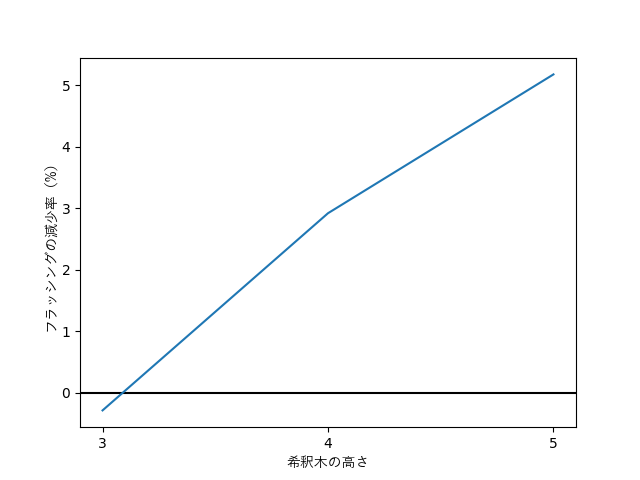
\includegraphics[scale=1.0]{img/decreasement.png}
 \caption{3,4,5のそれぞれの高さを持つ希釈木の,変形操作によるフラッシングの回数の平均削減率}\label{fig:graph}
\end{figure}
